\csname documentclass\endcsname[../main.tex]{subfiles}
\begin{document}
\chapter{Background and Related Work}
% sole purpose: what these people have done is not sufficient
% present it with my research question in mind
% eg when talking about rl, talk about previous work and how it connects to our work (which this connection has not yet been explored yet)
% figures: quality very important

In this chapter, we explain the background knowledge
for this project, including CBMs, CEMs, IntCEMs,
and other existing intervention policies. All existing 
intervention policies adopt a greedy approach to performing interventions,
whereas we hypothesise that non-greedy intervention policies can outperform greedy intervention policies.
We highlight how these existing greedy intervention policies is able to achieve competitive 
predictive accuracies,
but are insufficient
for learning a non-greedy
intervention policy for different budgets.

\section{Concept Bottleneck Models}\label{background:cbm}
For predictive tasks where an input (eg. an image of a medical scan)
is used to predict a label (eg. the presence of cancer),
practitioners can often explain their predictions
via high-level concepts, such as the presence of tumours,
changes in tissue structure, etc. However, 
most Machine Learning (ML) models do not have this kind of interpretability as they are trained to directly
predict labels from inputs.
Concept Bottleneck Models (CBMs), proposed by Koh et al.~\cite{cbm}, aim to increase the interpretability 
of ML models
by augmenting regular ML models with a set of $k$
human-interpretable concepts $\mathcal{C}$. These models learn to predict concepts from inputs, which are then used to predict a label.
Structurally, CBMs consist of a sub-model $g$ that learns a mapping from
input $\mathbf{x}$ to concepts $\mathbf{c}$, and we refer to $\mathbf{c}$
as the CBM bottleneck.
$\mathbf{c}$ is a vector representing the concepts present in the input, 
where each entry corresponds to the predicted probability of a concept being in the input.
CBMs contain another sub-model $f$
that learns a mapping from concepts $\mathbf{c}$
to the output label $\mathbf{y}$.
The overall structure is given by
\[g(\mathbf{x}) = \mathbf{c}, f(\mathbf{c}) = \mathbf{y}\]
Which is shown in Figure~\ref{fig:cbm}.
% These types of model can be created by simply adding a new layer in traditional models
% with the same number of activations as the number of concepts, where this layer
% is referred to as the bottleneck. 
Henceforth we refer to $g$ as the ``concept predictor $\mathbf{x} \to \mathbf{c}$ model'' and $f$ as the
``label  predictor $\mathbf{c} \to \mathbf{y}$ model''.
%  Training such a model requires a
% dataset of inputs $\mathbf{x}$ annotated with the corresponding 
% concepts $\mathbf{c}$ and labels $\mathbf{y}$. 

\begin{figure}[!ht]
    \centering
    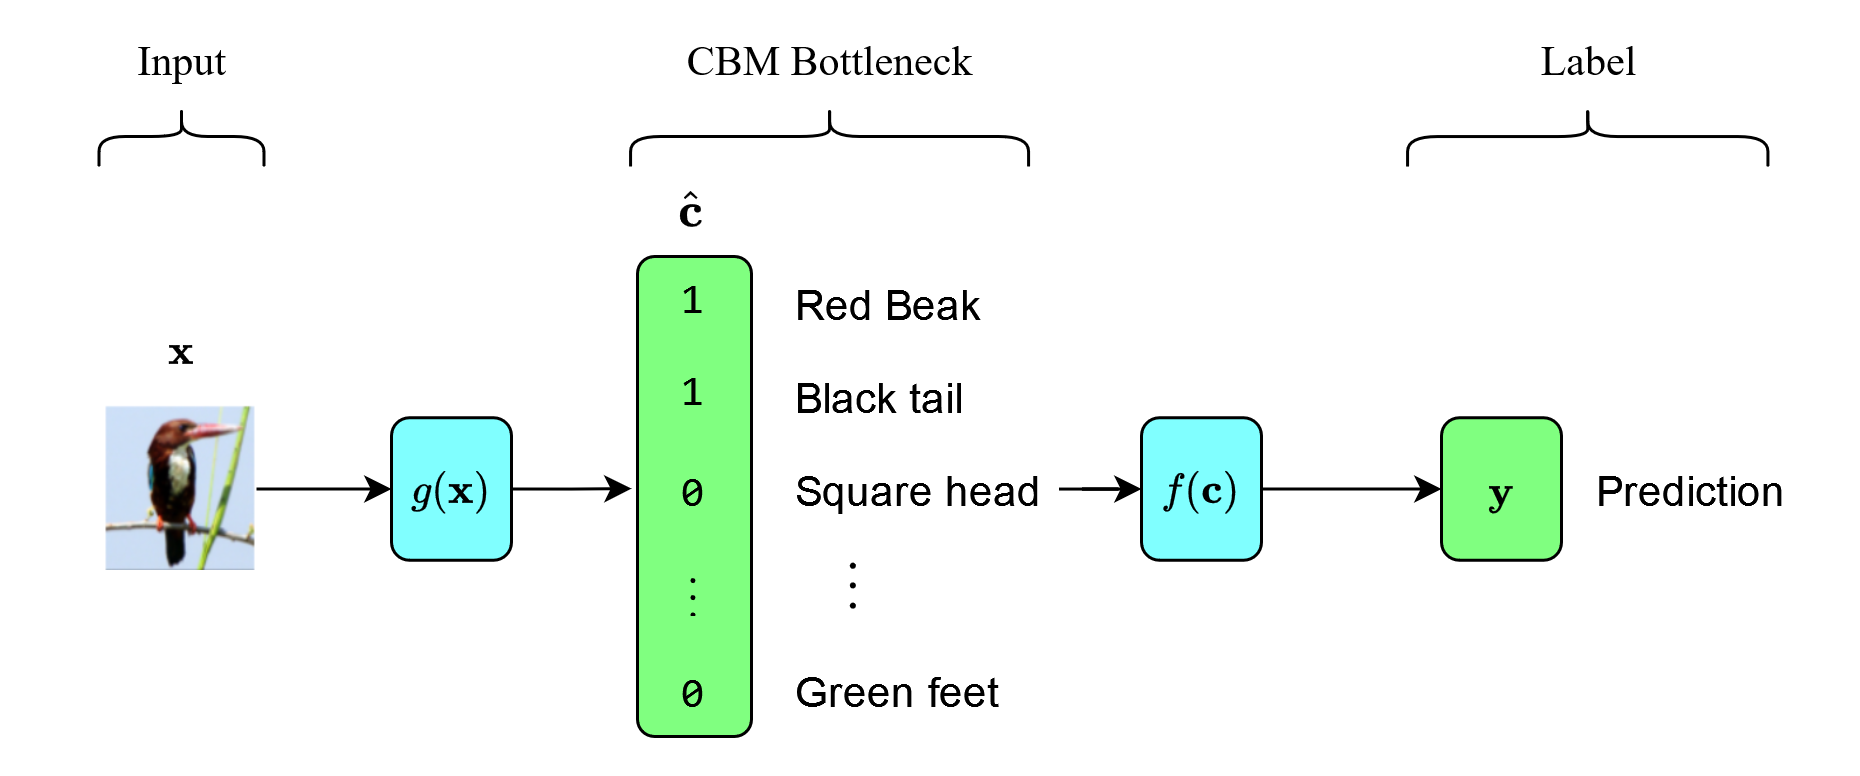
\includegraphics[width=0.8\textwidth]{figs/background/cbm.png}
    \caption{The Concept Bottleneck Model  Architecture~\cite{cbm}.}
    \label{fig:cbm}
\end{figure}

CBMs allow for interventions during 
inference time. Domain experts can 
perform interventions by correcting the intermediate concepts
predicted by the $\mathbf{x} \to \mathbf{c}$ model. This improves the performance of the $\mathbf{c} \to \mathbf{y}$ model,
which is illustrated in Figure~\ref{fig:cbm-interventions}.
To train a CBM, we utilize a combination of 
a concept loss $\mathcal{L}_{\text{concept}}$ that measures the
discrepancy between the predicted concepts $\hat{\mathbf{c}}$ 
and actual concepts $\mathbf{c}$, as well as a label loss $\mathcal{L}_{\text{label}}$
that measures the discrepancy between the predicted label $\hat{\mathbf{y}}$
and actual label $\mathbf{y}$.

\begin{figure}[!ht]
    \centering
    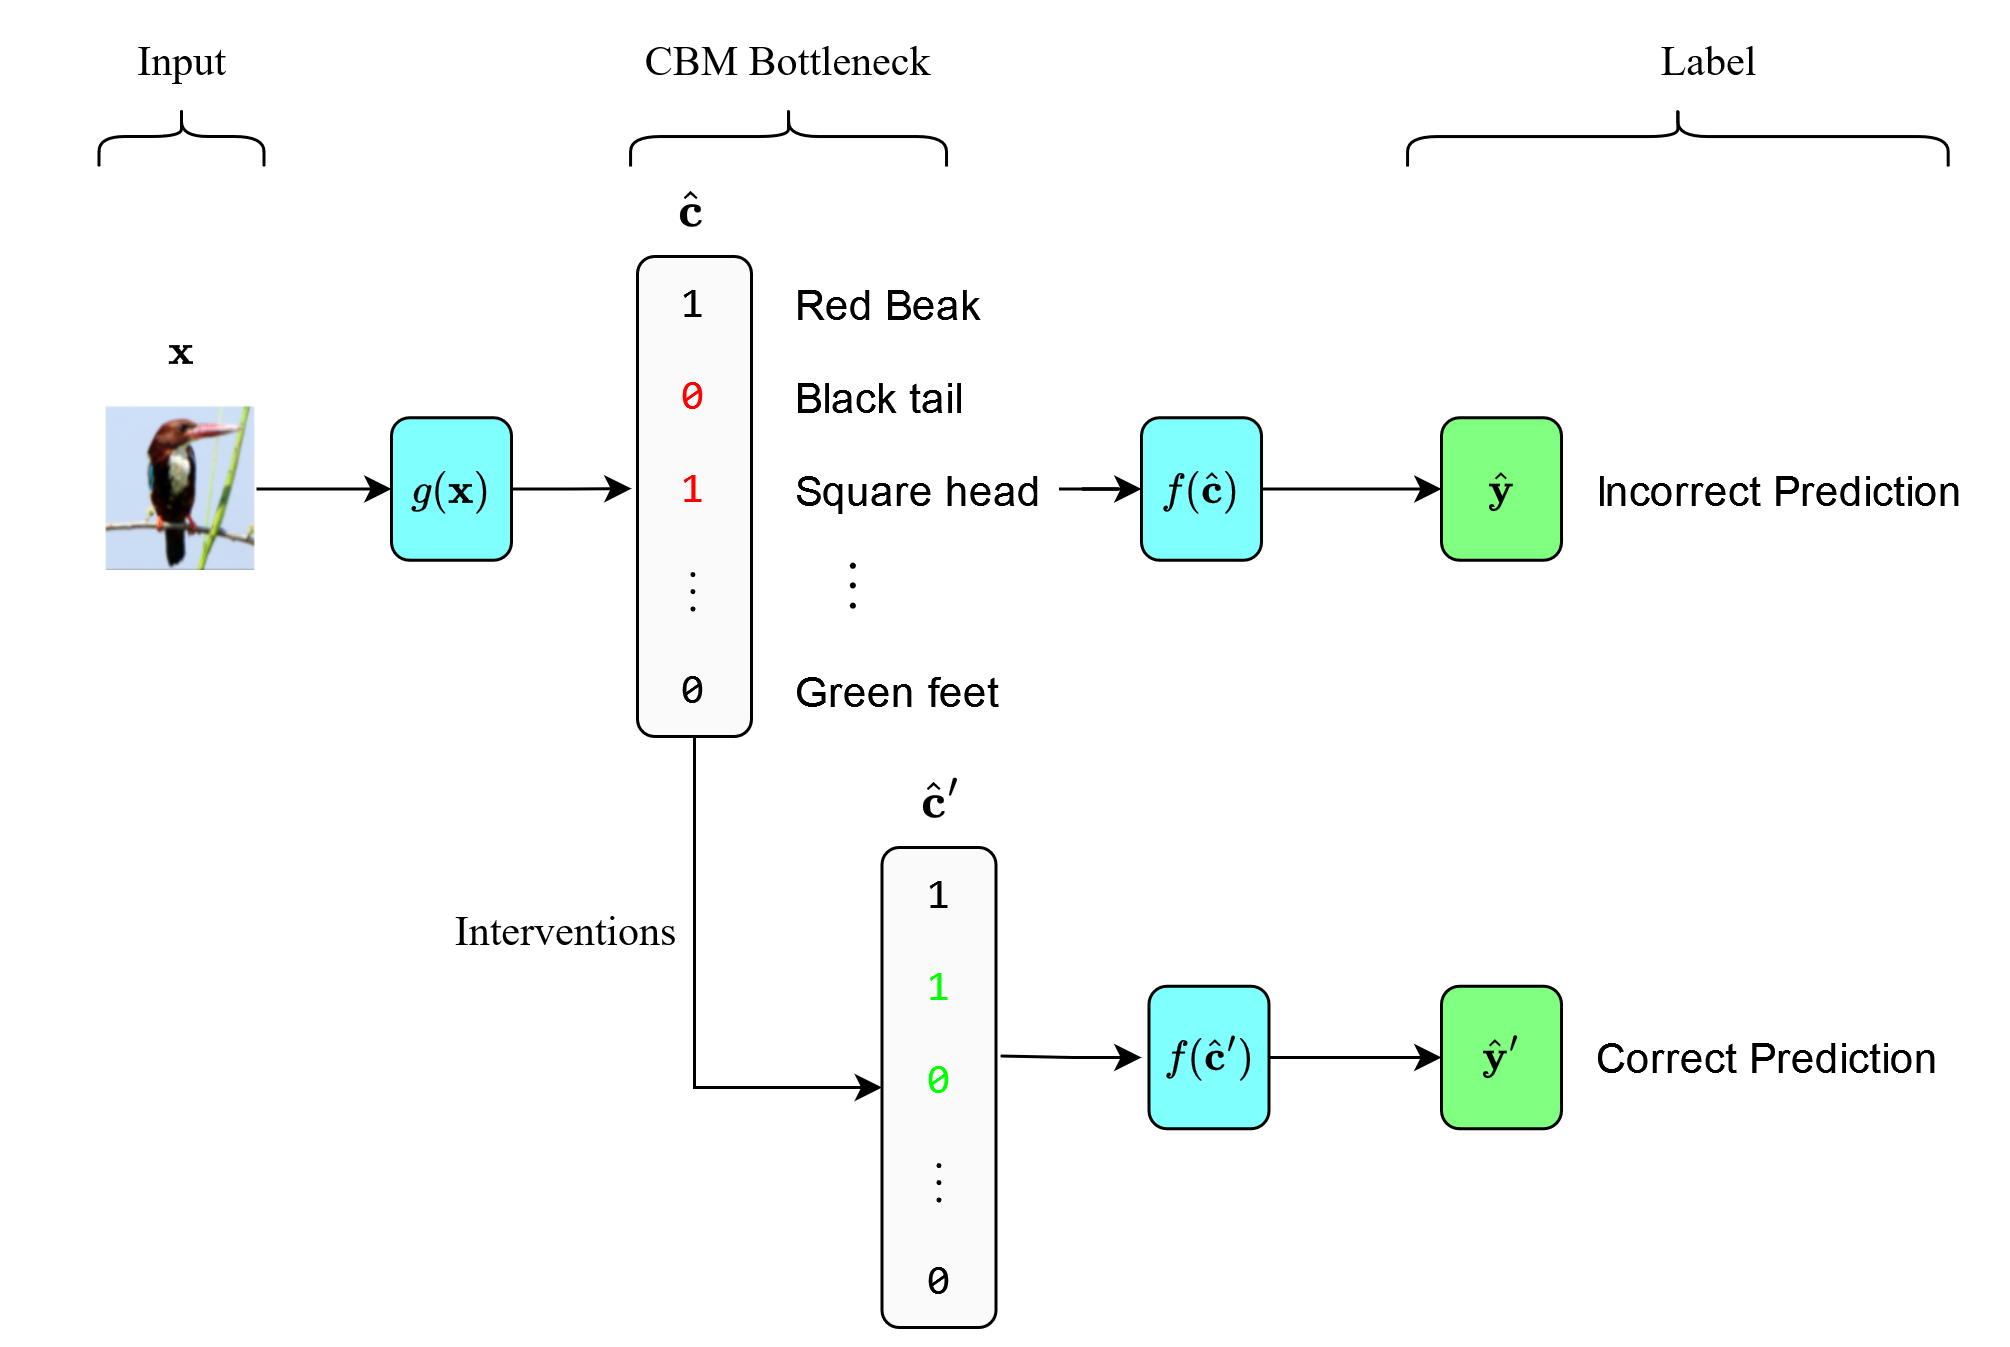
\includegraphics[width=0.8\textwidth]{figs/background/cbm_interventions.png}
    \caption{An illustration of intervening on the concepts predicted by a CBM.}
    \label{fig:cbm-interventions}
\end{figure}
% \subsection{Training CBMs}

% To train

% There are several different ways to train a CBM. 
% If we let the concept loss $\mathcal{L}_{\text{concept}}$ be a loss
%  function that measures
% the discrepancy between the predicted concepts $\hat{\mathbf{c}}$
% and the actual concepts $\mathbf{c}$, and similarly the 
% label loss $\mathcal{L}_{\text{label}}$ measuring the discrepancy
% between the predicted concepts $\hat{\mathbf{y}}$
% and the actual concept $\mathbf{y}$,
% both losses as illustrated in Figure~\ref{fig:cbm}.
% There are the following ways
% to train a CBM as proposed in~\cite{cbm}.

% \begin{enumerate}
%     \item Independent: Training the two models independently by minimizing
%     $\mathcal{L}_{\text{concept}}(g(\mathbf{x}), \mathbf{c})$ and $\mathcal{L}_{\text{label}}(f(\mathbf{c}), \mathbf{y})$ independently.
%     \item Sequential: Training the models one by one, first learning
%     $\hat{g}$ by minimizing 
    
%     $\mathcal{L}_{\text{concept}}(g(\mathbf{x}), \mathbf{c})$,
%     then learning $f$ by minimizing $\mathcal{L}_{\text{label}}(f(\mathbf{\hat{g}(\mathbf{x})}), \mathbf{y})$
%     \item Joint: The model is trained via a weighted sum of the losses given by \\ 
%     $\lambda_{\text{concept}} \mathcal{L}_{\text{concept}}(g(\mathbf{x}), \mathbf{c}) + \lambda_{\text{label}} \mathcal{L}_{\text{label}}(f(g(\mathbf{x})), \mathbf{y})$ \\
%     such that both losses are minimised simultaneously.
% \end{enumerate}

% It has been shown experimentally that while the joint models perform the best
% without interventions, followed by the sequential model, and the independent model
% performs the worst. This is because the sequential model allows the $\mathbf{c} \to \mathbf{y}$ 
% model to learn a mapping from the concepts produced by the $\mathbf{x} \to \mathbf{c}$ model to
% label $\mathbf{y}$, where the concepts produced by the $\mathbf{x} \to \mathbf{c}$ model is often different
% from the true concepts, an underlying requirement for the independent model to perform well. Additionally,
% the joint model allows the $\mathbf{x} \to \mathbf{c}$ model to simultaneously learn to output a representation
% of concepts that allow for best performance of the $\mathbf{c} \to \mathbf{y}$ model~\cite{cbm}.

% When comparing performance under interventions,
% independent models outperform the two models.
% They are more sensitive to interventions and each successive intervention step
% leads to a bigger increase in performance compared to the other two,
% with better performances after the same number of interventions.
% The reason behind this
% is that the independent model learns a mapping from the true concepts to the label,
% whereas the other two learn a mapping from the predicted concepts to the label. Each intervention
% modifies the predicted concepts to be closer to the true concepts, which is what the 
% $\mathbf{c} \to \mathbf{y}$ independent model is trained to do~\cite{cbm}.

\section{Concept Embedding Models}\label{background:cem}

While CBMs achieved
interpretability advantages, they do not perform as well as traditional ML models~\cite{cbm}. 
This is because of concept incompleteness,
which is when the annotated set of concepts in a dataset do not contain all concepts that can be extracted from the input for label prediction. Since the label predictor model
relies on the predicted concepts, concept incompleteness results in a loss of information and poor predictive accuracy.
This limits
the performance of the model as traditional models can extract
information outside these concepts~\cite{cbm-hybrid}. 
% This is even more apparent
% if the dataset does not contain a complete set of concepts that cover all
% features that can be used to predict the label, which is common in real life.
% As such, there is a trade-off between performance and interpretability, where researchers
% have developed methods such as extending the CBM bottleneck with a set of unsupervised neurons
% to increase accuracy at a cost of decreasing interpretability.

To overcome this trade-off
between performance and interpretability, 
Concept Embedding Models (CEMs) were proposed by Zarlenga et al.~\cite{cem}.
CEMs utilise learnable embeddings to replace the original CBM bottleneck,
learning two embedding vectors for each concept: one for
when the concept is present
and one for when the present is not.
% these are CBMs that further add an additional layer of learnable embeddings before
% the original bottleneck, 
% The architecture of CEMs is shown in Figure~\ref{fig:cem}.
% An intermediate scoring function $\phi_i$ is learnt for each concept $i$, 
% and the embedding assigned to the bottleneck is an interpolation of the two embeddings
% based on the scoring function predicting the possibility of the concept to be present.
% to increase the performance of CEMs, the authors utilised observations mentioned in
% Section~\ref{background:cbm}, where models trained on the true concepts are more sensitive to 
% interventions. They proposed RandInt, a method to randomly intervene
% during training with $\lambda_{\text{int}} = 0.25$ probability of intervening
% on a concept. They show that this effectively boosts the performance of the model 
% under interventions during test time without notable effects to the performance 
% without interventions~\cite{cem}.

CEMs successfully solve the trade-off problem between performance and interpretability,
allowing for similar performance to traditional models while maintaining the
interpretability, along with high concept accuracy. This is because the embeddings
encode more information
in the concept representations, for example, information
related to concepts not present in the dataset.
% The additional information present
% in the embeddings allow the task predictor model to 
% This is referred to as 
% concept leakage, where
% The additional information in the CEM bottleneck
%  compared to binary representations in CBMs
% lead to a better performing label predictor model.
% CEMs are still trained 
% on the same set of human-interpretable concepts as CBM via a similar concept loss, which leads to
% high interpretability and good intervention performance.
 It has been shown experimentally
that CEMs achieve better predictive accuracy than CBMs,
especially for 
concept-incomplete dataset tasks (where
the annotated concepts
do not cover all concepts present in input).
Additionally these learnt concept
embedding representations effectively represent the true concepts measured by an alignment score~\cite{cem}.

This architecture also allows for interventions during test-time. By simply replacing
the output of the concept predictor model with the embeddings that represent
the true concepts, we can correct the concept predictions
 and improve the performance of the model. 


\section{Interventions}
A key advantage of using CBMs is having access to 
test-time interventions, which is the idea of utilizing experts
to modify incorrect concept predictions to improve the 
performance of the model.
For simplicity, assume that
all interventions are correct,  
and an intervention is defined by 
modifying a concept prediction to its ground truth value
. To formalize interventions, we define
them via the following function, where
the predicted concepts $\hat{\mathbf{c}}$ and the true concepts $\mathbf{c}$ are interpolated
using a binary intervention vector $\bm{\mu}$.

\begin{equation}\label{equation:intervention}
I(\hat{\mathbf{c}}, \mathbf{c}, \bm{\mu}) = 
\bm{\mu} \; \mathbf{c} + (1 - \bm{\mu}) \; \hat{\mathbf{c}} \qquad \hat{\mathbf{c}} \in [0,1]^k, \mathbf{c}, \bm{\mu} \in \{0, 1\}^k
\end{equation}

Figure~\ref{fig:interventions} demonstrates how an intervention
is formed using 
a binary mask $\bm{\mu}$ from the predicted concepts $\hat{\mathbf{c}}$ and the true concepts $\mathbf{c}$.

\begin{figure}[!ht]
    \centering
    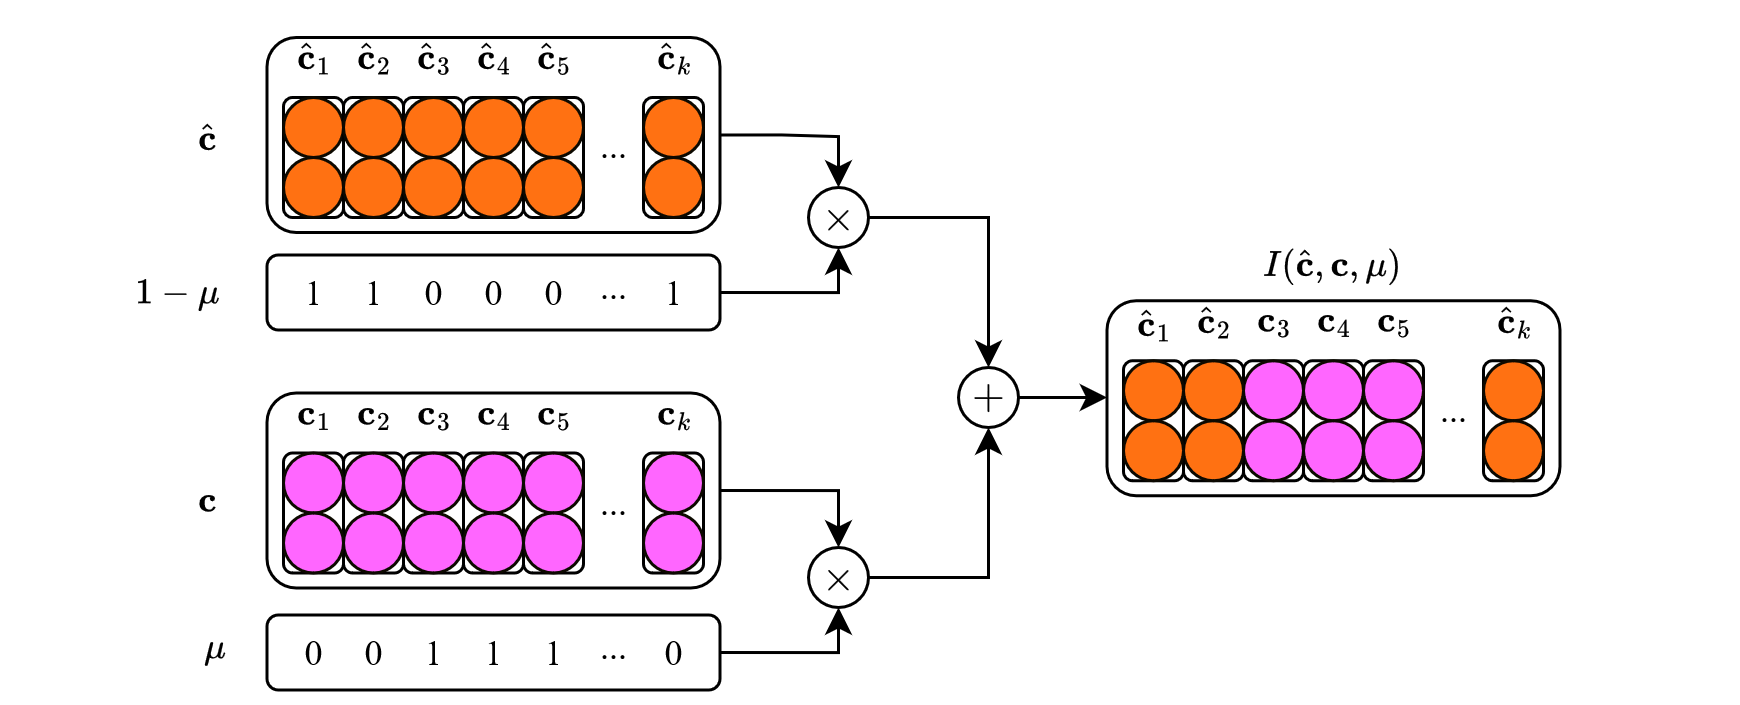
\includegraphics[width=\textwidth]{figs/method/interventions.png}
    \caption{An example of how interventions are formed from the predicted concepts $\hat{\mathbf{c}}$
    and true concepts $\mathbf{c}$
     using binary mask $\bm{\mu}$.}
    \label{fig:interventions}
\end{figure}

\subsection{Intervention Policies}
Since it is infeasible to ask experts to intervene on all concepts,
intervention policies were developed to 
generate an ordering for concept interventions,
usually with the goal of maximising the post-intervention 
predictive accuracy of the $\mathbf{c} \to \mathbf{y}$ model. 
As shown in~\ref{equation:greedy-intervention-policy},
an intervention policy $\mathcal{P}$ generates the next concept $c_i$ to be intervened on, given the previously
intervened concepts $\bm{\mu}$ and 
predicted concept probabilities $\hat{\mathbf{p}}$~\cite{ectp, coop, intervention-policies}.
\begin{equation}\label{equation:greedy-intervention-policy}
\mathcal{P}(\bm{\mu}, \hat{\mathbf{p}}) =c_i
\end{equation}
Most current greedy intervention policies
either select the concepts that 
minimise uncertainty~\cite{coop, ectp}, 
or directly learn a greedy 
intervention policy
by mimicking the behaviour of an oracle
policy that has access to the ground truth labels $\mathbf{y}$ at test-time~\cite{behavioural-cloning, intcem}.
Non-greedy intervention policies
are different in that they output a set of concepts to be intervened on given a budget,
which we further discuss in Section~\ref{method:non-greedy-policies}.
% A greedy intervention policy $\mathcal{P}$
% is a collection of functions $\mathcal{P}_i$, each
% of which outputs the concept to intervene on at step $i$. An optimal greedy policy is the following

% \[\hat{\mathcal{P}} = \mathop{\mathrm{argmin}}_{\mathcal{P}} \sum_{j = 1}^{k} \mathcal{L}_{\text{label}}(\hat{g}(\hat{\mathbf{c}}_{\mathcal{P}, j}), \mathbf{y}) \]
% \[\hat{\mathbf{c}}_{\mathcal{P}_0} = \hat{\mathbf{c}}, \hat{\mathbf{c}}_{\mathcal{P}_j} = I(\hat{\mathbf{c}}_{\mathcal{P}_{j-1}}, \mathbf{c}, \mathcal{P}_j(\hat{\mathbf{c}}_{\mathcal{P}_{j-1}}))\]
% Which maximizes the accuracy at each step $j$ sequentially
% for all $k$ concepts. At each
% step, $\hat{\mathbf{c}}_{j-1}$ is 
% the predicted concept after the previous $j-1$ interventions,
% and we aim to maximize the accuracy of the prediction made by the
% $\hat{g}: \mathbf{c} \to \mathbf{y}$ model.
% While existing work focuses on 
% greedy intervention policies to develop an order for concepts to intervene, whereas a non-greedy intervention policy 


\section{Intervention-Aware Concept Embedding Models} % 500

Building on top of CEMs, Zarlenga et al.~\cite{intcem} introduced 
Intervention-aware CEM (IntCEM), CEMs that are augmented
with machine learning model
that learns a concept intervention policy. IntCEMs' novelty
lies in framing the problem of training a CEM and finding
an intervention policy as a joint optimisation problem by augmenting
existing CEMs with a trainable intervention policy model $\psi$. 
This approach offers significant improvements in performance after 
interventions while maintaining similar performance without 
interventions. 
IntCEM achieves this as it directly uses an ML
model $\psi$ to
learn to mimic the behaviour of an oracle
greedy intervention policy, 
and the CEM is also trained to be more sensitive to interventions
by the model. 
% Thethe introduction of an intervention loss 
% $\mathcal{L}_{\text{intervention}}$ and label loss $\mathcal{L}_{\text{label}}$ for 
% the intervened concepts.


The overall training loop of IntCEM 
is shown in Figure~\ref{fig:intcem}.
During training, $\psi$ first samples intervention
logits $\omega$ for the next concept to intervene on.
To train $\psi$ to mimic 
the behaviour of an oracle 
greedy intervention policy $\psi^*$ that has access to the true
labels, we find the output of $\psi^*$
by searching over all concepts to find the one that 
leads to the highest increase in predictive accuracy.
We then compute an intervention loss $\mathcal{L}_{\text{intervention}}$ to minimize the discrepancy between the outputs of $\psi$ and $\psi^*$.
This is referred to as Behavioural
Cloning~\cite{behavioural-cloning}.

Koh et al.~\cite{cbm} demonstrated that
training the $\mathbf{c} \to \mathbf{y}$ model using ground
true concept labels increase the model's sensitivity
to interventions,
leading to better intervention performance.
IntCEM incorporates this idea by 
also using 
the post-intervention concepts to
computing the label loss $\mathcal{L}_{\text{label}}$.
Not only does this increase the model's sensitivity to interventions,
it specifically increases the model's sensitivity to interventions
sampled by $\psi$ to further improve its intervention performance. At each intervention step,
the intervention mask $\bm{\mu}$ is updated according to 
the next concept to intervene $\eta$ sampled from $\psi$.

The final loss is computed as a weighted average of the three losses,
given by 
\[\mathcal{L} = \lambda_{\text{concept}} \mathcal{L}_{\text{concept}}
+  \lambda_{\text{label}} \mathcal{L}_{\text{label}}
+  \lambda_{\text{intervention}} \mathcal{L}_{\text{intervention}}\]
Which is then used to update both the CEM and the intervention policy model $\psi$.

\begin{figure}[!ht]
    \centering
    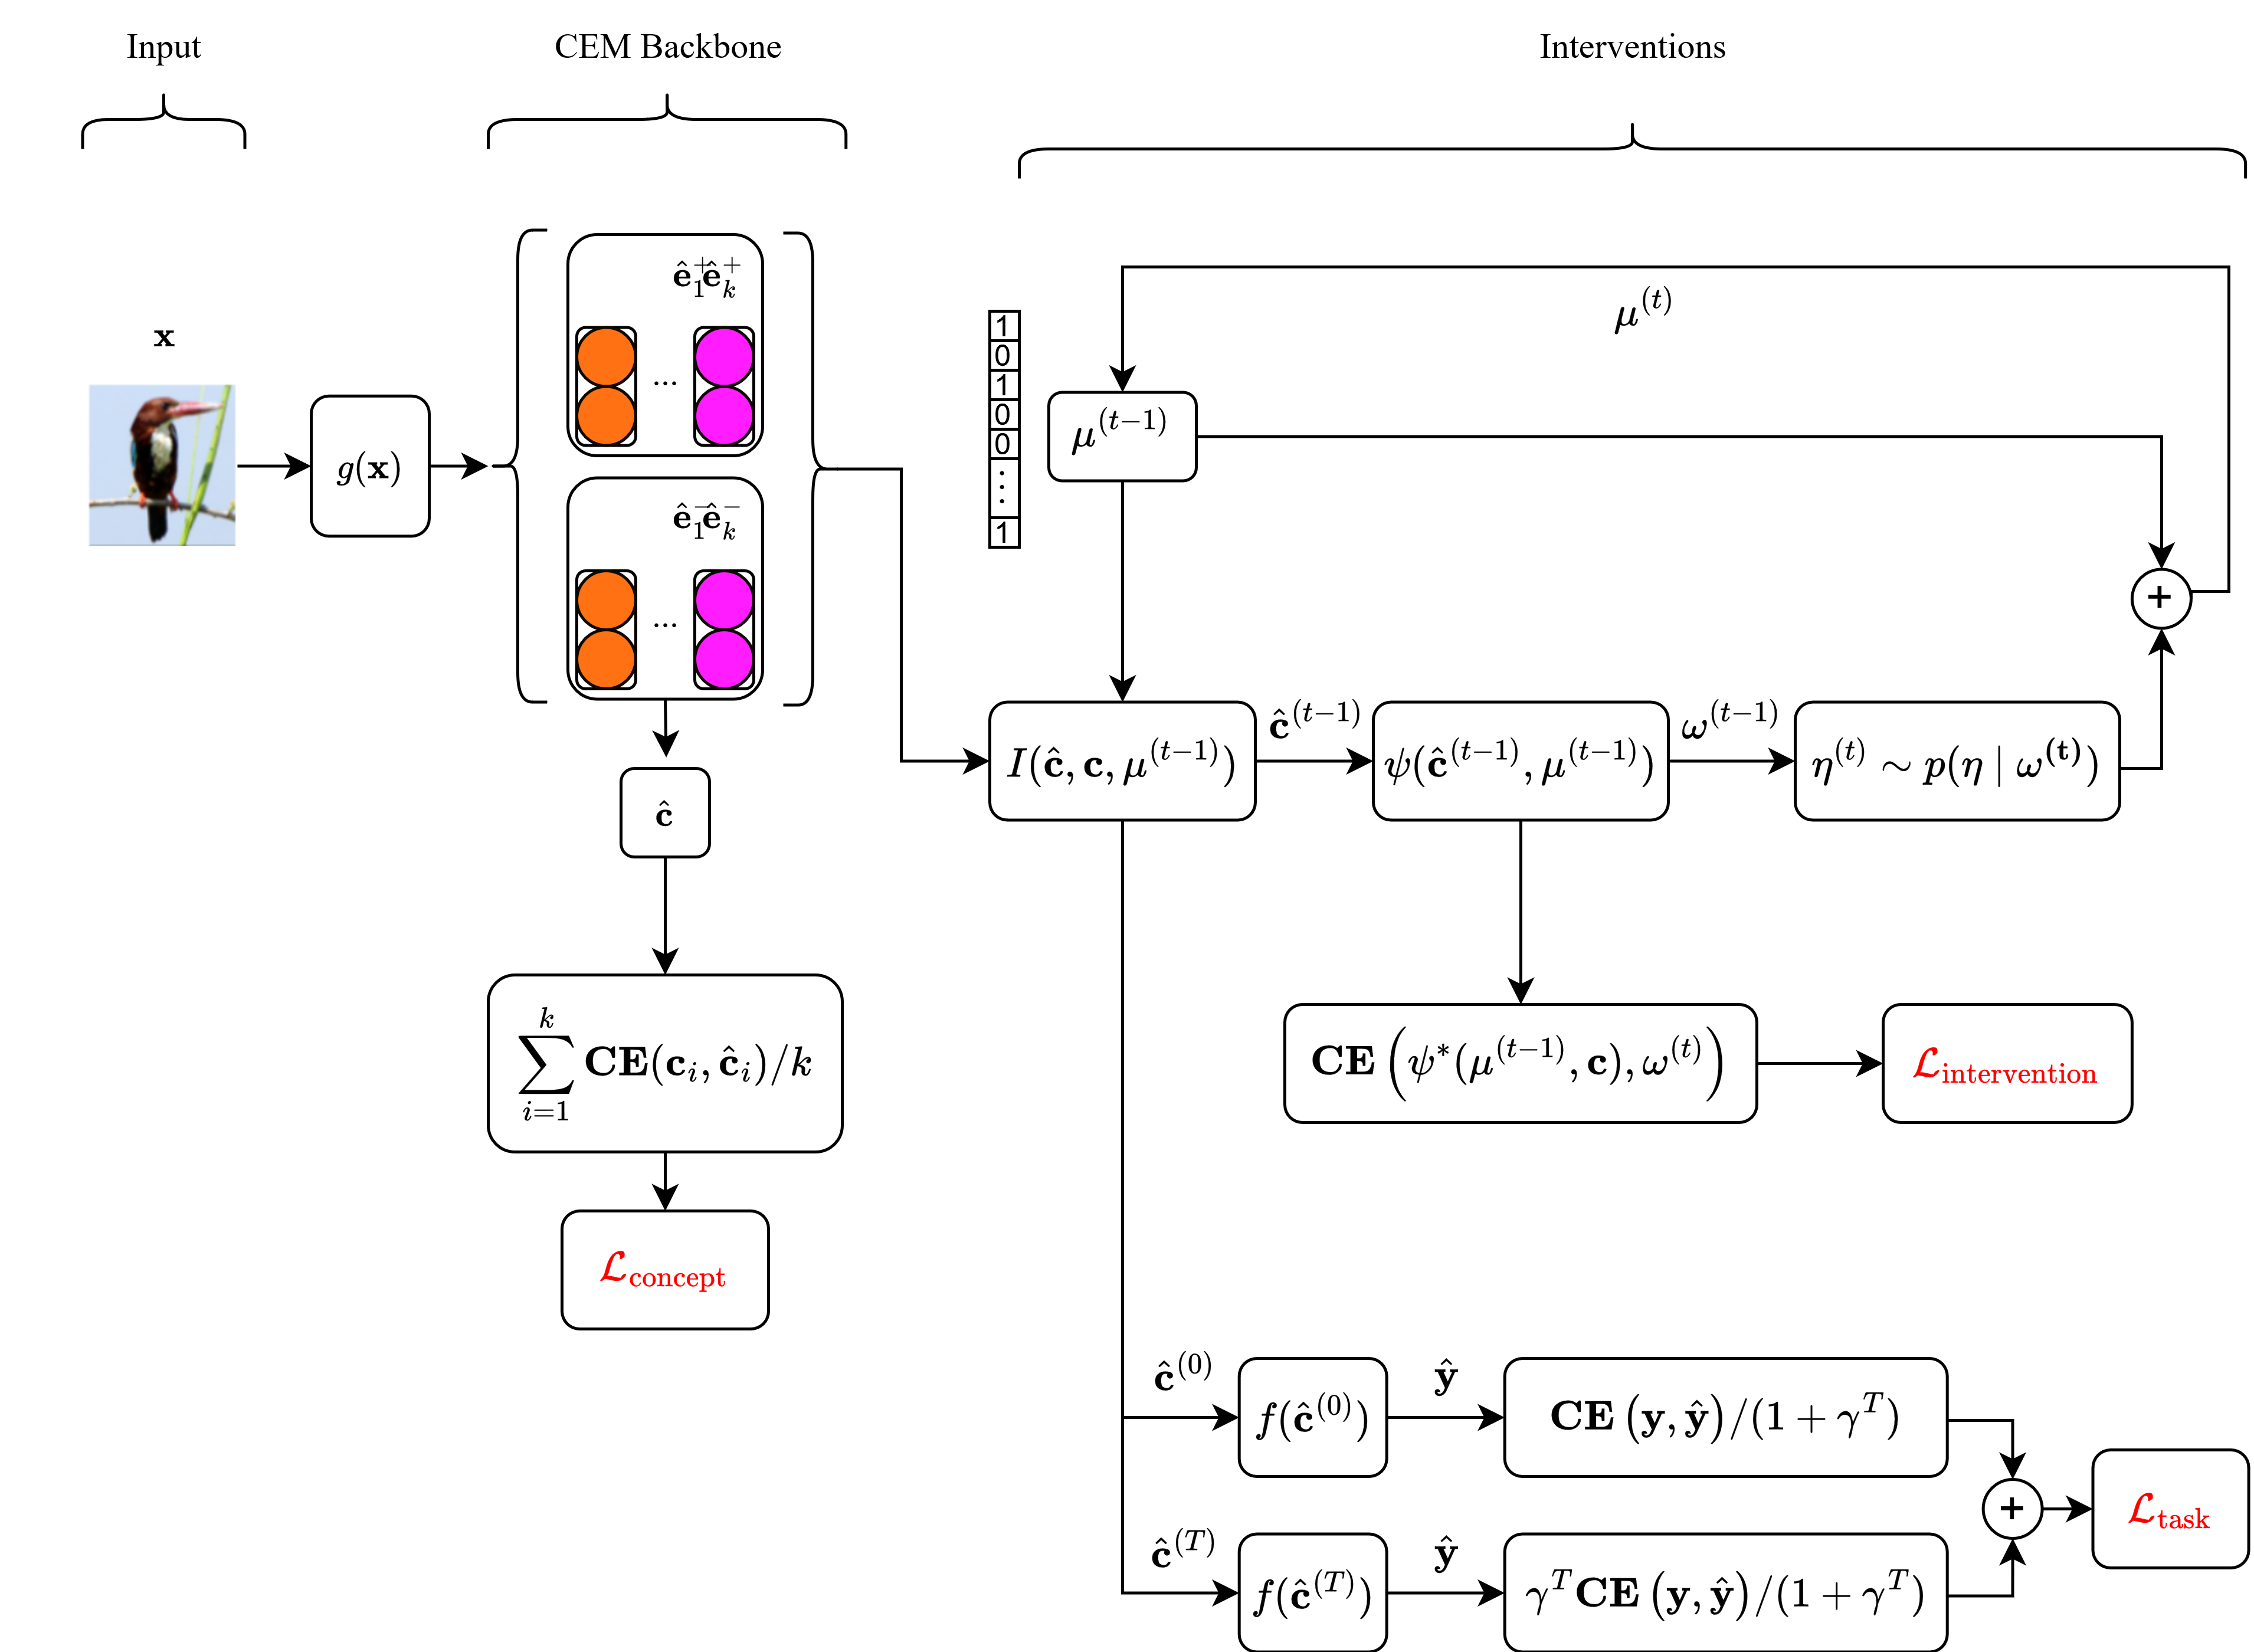
\includegraphics[width=\textwidth]{figs/background/intcem.png}
    \caption{The training loop of IntCEM. $\bm{\mu}$ is the intervention binary mask,
    $\eta$ the next concept to intervene on, and $\psi$ the intervention policy model.
    The loop computes concept loss $\mathcal{L}_{\text{concept}}$,
    intervention loss $\mathcal{L}_{\text{intervention}}$, and label loss $\mathcal{L}_{\text{label}}$ which is used to update the
    IntCEM.}
    \label{fig:intcem}
\end{figure}

Despite IntCEM's improved intervention performance,
we note that it learns a greedy intervention policy.
That is, its learnt policy tries to maximise the 
post-intervention accuracy at each step, 
by mimicking the behaviour of a greedy optimal policy. 
Non-greedy policies that utilise
Reinforcement Learning~\cite{rl} have seen a lot of
success in similar problems that require
making sequential decisions to maximise a performance metric at the end,
outperforming their
greedy counterparts~\cite{non-greedy-3, gsmrl, non-greedy-2, non-greedy-1}.
This is because these problems can be formulated as a Markov Decision Problem,
which Reinforcement Learning can be used to find a non-greedy policy for.
Therefore we propose that
non-greedy intervention policies can outperform greedy intervention policies
for different budgets as the optimal intervention sequence can differ when the budget
varies. 
If we were to adopt a similar approach to IntCEM by mimicking the behaviour of a 
non-greedy optimal policy,
at each step we would have to search through
$O(k!)$ combinations of concepts
to find the optimal set of concepts to intervene on for 
$k$ concepts. This is much larger
than the $O(k)$ searches required by the optimal greedy policy.
Therefore, trying to mimic the behaviour of a non-greedy oracle policy is infeasible due to the high time complexity.
As such, we cannot adopt a similar approach to learn a non-greedy intervention policy that maximises predictive accuracy for different budgets.
This prompts us to use Reinforcement Learning as an alternative approach.

\section{Reinforcement Learning}\label{background:rl} % 500
Reinforcement Learning (RL)~\cite{rl} focuses on
 training agents to make sequential decisions in an environment.
% Contrary to supervised learning
% where the goal is to minimize the discrepancy between predicted outputs and true outputs,
where the goal is to maximise the cumulative rewards received by the agent
by taking actions over time. 
RL aims to solve a Markov Decision Problem, which consists of a set of states $\mathcal{S}$, 
actions $\mathcal{A}$, and 
a transition function $t: \mathcal{S} \times \mathcal{A} \to \mathcal{S}$
that tells us how states transition to new states.
The agent has access to observations which reflect the current state
 of the environment and can take actions to progress to different states until termination.

In this project, we utilise Reinforcement Learning 
to learn a non-greedy policy to decide which
concepts to intervene. We select
 the Proximal Policy Optimization~\cite{ppo}
algorithm to do this, a SOTA policy-based RL algorithm which has shown to be robust 
and perform well in many different Reinforcement Learning problems~\cite{ ppo-2, ppo-1, ppo-3}.
% combines the strengths of traditional policy-based~\cite{trpo}
% approaches
% and value-based approaches~\cite{deep-q-learning, deep-q-learning-2}.
PPO aims to train the agent to learn a policy $\pi$ that takes the current state from the environment as input,
and outputs probabilities for each action it can take.
The goal of the policy
is to output higher probabilities for actions that have higher rewards.
In PPO,
the Agent is defined by an Actor model $\theta$ and a Critic model $\phi$.
The Actor model learns a policy $\pi_\theta$ and decides on what actions to take based on 
the current state.
The Critic model learns 
to estimate the value $V_\phi(s)$ of a current state, which is an estimation of the sum of all future rewards, each of which is discounted 
by a factor $\gamma_{RL}$ according to how 
far in the future the reward is.
This also gives us the next state value function $Q_\phi$ 
based on rewards
and the approximation from $V_\phi$,
which is the value of taking an action 
\begin{equation}\label{equation:next-stat-}
Q_\phi(s,a) = 
r + \gamma_{RL} V_\phi(s')
\end{equation}
equal to the reward $r$ and value 
of the next state $s'$ discounted by $\gamma_{RL}$.
We can then also compute
an advantage function $A_\phi(s,a) = Q_\phi(s,a) - V_\phi(s)$
that estimates the advantage of taking an action.

During training, we have states $s_i$, 
and we sample actions $a_i$ from the Agent
and obtain the corresponding reward
from the RL environment.
We then repeat using the new state $s_{i+1} = t(s_i, a_i)$ until we reach the termination state.
This allows us to compute 
the next state value function,
then used to compute a value loss $\mathcal{L}_{\text{value}}$ for the Critic model
to minimise the discrepancy between the estimated and true
values, using the following equation
\begin{equation}\label{equation:rl-loss}
\mathcal{L}_{\text{value}} = \frac{1}{k} \sum_{i=0}^k 
\nabla_\phi (V_\phi(s_i) - Q_\phi(s_i,a_i))
\end{equation}
We can also compute a policy loss $\mathcal{L}_{\text{value}}$ for the Actor model
to update it in the direction that maximises the advantages
computed using the Values estimated by the Critic model
\[\mathcal{L}_{\text{policy}} = -\frac{1}{k} \sum_{i = 0}^k \nabla_\theta \log
 \pi_\theta(a_i \mid s_i) \cdot A_\phi(s_i, a_i)\]

Since the Actor model
maximizes the advantages based on the Value function
estimated by the Critic model,
this allows the 
RL agent to balance between exploration and exploitation.
Initially the Actor model explores states which may have low true values
which are not learnt by the Critic model, and as the Critic model
learns to estimate the values of states better, the Actor model also 
learns a better policy~\cite{ppo}. Apart from the Actor and Critic models,
PPO also utilizes
a clipping function to prevent the policy update 
from being too large or too small.
Section~\ref{method:rl} goes into how
the PPO algorithm is used to train an RL agent that learns 
a non-greedy intervention policy.
 
\section{Flow Models}\label{background:flow}
Flow models model probability distributions by leveraging the change of variable property~\cite{normalizing-flows}.
Given an input random variable $X$,
if we can define an invertible transformation function $f$ such that
$f(X) = Z$ and $f^{-1}(Z) = X$ for another random variable $Z$,
the change of variable property says that 
the probability densities of the two random variables $p_X$ and $p_Z$,
are related in the following way:
\begin{equation}\label{equation:change-of-variable}
p_X(x) = \left | \mathop{\mathrm{det}} \frac{d f^{-1}(x)}{d x}
\right | p_Z(f^{-1}(x))
\end{equation}
using the Jacobian determinant of the inverse of $f$.

Flow models define transformations
using ML models with this property with learnable parameters.
These transformations are designed to be easily invertible
and which the Jacobian determinant is simple to calculate.
These transformations can be composed by sequentially applying them,
and the probability distribution can also be found by sequentially
applying Equation~\ref{equation:change-of-variable}.

During training, a latent distribution is chosen
which is usually one with a 
probability density that is simple to sample from.
These transformations, which when composed can be used to 
transform the simple latent distribution a more complex distribution,
are then used to model the complex data distribution, such as 
the distribution of concepts within a dataset for CEMs. This allows 
us to model and sample from distributions which would otherwise 
be difficult to sample from.
Section~\ref{method:surrogate} explains how we utilize a variation of 
these normalizing flow models to model the conditional distribution of concepts,
which is then used to provide intermediate rewards for the RL agent 
to learn a non-greedy intervention policy.

\section{Related Work}

\subsection{Expected Change in Target Prediction}\label{background:ectp}
Expected Change in Target Prediction (ECTP)~\cite{ectp} is a greedy 
intervention policy that selects at each step, the concept which 
when intervened, leads to the largest change in the probability
of the currently predicted class. This is because this concept
is the most ``important'', and mis-predicting this concept
will result in the largest increase in label error. This can be 
summarised as a score, for predicted concepts $\hat{\mathbf{c}}$
and $\hat{\mathbf{y}}$, the importance score of a concept $c_i$ is given by
\[\mathbb{E}_{v \sim p_g(c_i \mid \mathbf{x})} 
[p_f(\hat{\mathbf{y}} \mid c_i = v, c_{\backslash\{i\}})] - p_f(\hat{\mathbf{y}} \mid c_i, c_{\backslash\{i\}})
\]
taking over expectation of the distribution of values of $c_i$
which takes over expectation of the distribution of values it can change to,
using the probabilities computed by the concept predictor model
$g$ and label predictor model $f$.


ECTP is a greedy intervention policy which selects the 
concept with the highest importance to intervene on,
and thus does not answer our research question.

\subsection{CooP}\label{background:coop}
Cooperative Prediction (CooP)~\cite{coop} 
further builds on the idea of ECTP and utilizes
uncertainty as an additional metric for cooperative prediction of 
concepts to intervene.
CooP is a greedy intervention policy that 
uses a score function,
selecting concepts with the highest score at each step
to intervene.
Its score function consists of a combination of the concept prediction
uncertainty, the concept importance score and acquisition cost.
The concept prediction uncertainty for a concept $c_i$
and a given input $\mathbf{x}$ is calculated by the entropy
of the distribution
\[H [p_\theta(c_i \mid x)] \]
which measures the expected information gain.

It uses a weighted sum of this information gain score,
the concept importance score mentioned in Section~\ref{background:ectp},
and the acquisition cost, which are the three factors believed that 
makes a concept optimal for interventions
. For simplicity we assume that all concepts have the same acquisition cost.

However, this does not answer our research question as
\begin{enumerate}
    \item It is a heuristic-
    based intervention policy, and we aim to find a learnt intervention
    policy which has been shown to have better performance on different 
    datasets.
    \item It is a greedy intervention policy. We think that non-greedy
    policies can outperform greedy ones, thus we believe there are better
    approaches that we aim to investigate.
\end{enumerate}

As shown in Section~\ref{method:surrogate},
we also use an uncertainty-based
idea to guide the Reinforcement Learning agent.
We utilise the expected information gain to the target variable
as intermediate rewards to the RL agent, with the goal of guiding it to 
perform interventions that will maximize the information gain, reducing
uncertainty and learning a non-greedy intervention policy model
that maximizes the post-intervention predictive accuracy. We compare 
the performance of our approach against CooP in Section~\ref{eval:rlcem-performance}


\subsection{Active Feature Acquisition}\label{background:afa}
Active Feature Acquisition (AFA)~\cite{afa} is the problem of deciding
what features to acquire from the environment, dynamically based
on their expected utility and acquisition cost, in order to 
improve predictive performance. Compared to
CBMs and interventions, AFA focuses on 
the trade-off between the benefit and costs of acquiring concepts,
specifically cost-efficiency, whereas
CBMs focus on predicting human-interpretable concepts 
from input. While these two focus on different field and aspects
of Machine Learning, we can draw a parallel between
interventions in CBMs and acquiring features in AFA.
Intervening on concepts is similar to acquiring features in AFA,
where this allows us to learn about the true values of them,
and the two both have the same goal of maximizing predictive performance.
However, our problem of interventions is more complex as we have to take
into account the original prediction by the CBM and budgets for interventions.
Reinforcement Learning has been applied to AFA to learn a non-greedy
policy for acquiring features, and has shown impressive results
in determining good feature acquisition policies.
In Section~\ref{method:rlcem} we look into how we can apply ideas of using
RL in AFA to learn a non-greedy intervention policy.

% discuss more work on intervention policies
% consider having AFA as its own section

In this chapter, we have explained the 
background for this project, as well as why existing research
does not answer our research question. In the next section
we look at our proposed solution and how it answers our research question.

\end{document}